% !TeX root = ../sustechthesis-example.tex

\chapter{蛇形结构后屈曲行为的调控}
\section{引言}
上一章研究了蛇形结构的分岔行为以及多稳态行为。该结构在实际应用中,特别是在柔性电路中的应用,往往需要根据实际情况来优化蛇形结构的几何参数。本章将提出一种优化蛇形结构后屈曲行为的方法并给出相应的优化结果。具体而言,通过优化结构的几何参数来实现对结构在后屈曲阶段分岔点位置的控制,从而实现对结构非线性行为的调控。本章首先介绍优化目标函数的设计,以及所用的优化方法及其相应的工具包。随后展示优化结果,结果可分为三部分:对于单单元蛇形结构($n_c=1$)而言,通过优化蛇形结构的厚度分布来调控结构屈曲模态交换的临界高度及相应交换临界载荷。对于双单元蛇形结构($n_c=2$)而言,本章通过优化蛇形结构中各直条带的长度,来实现双单元蛇形结构中的模态交换,并对优化后结构进行详细的分岔分析来阐明在双单元蛇形结构的屈曲模态交换过程中同样存在多重特征值分岔来实现稳定性的交换。最后,对三单元蛇形结构($n_c=3$)而言,本章通过调控不同单元的厚度,来说明通过单元厚度的调节可以有效影响屈曲构形。
\section{结构优化方法}
本节给出用于优化蛇形结构后屈曲行为的目标函数的设计思路,所使用的优化算法以及具体的优化程序。

蛇形结构在临界拉伸载荷下会发生面外屈曲,该临界载荷对应于一个超临界分岔点。进入后屈曲阶段后,一方面,原平面分支上会出现二阶屈曲模态对应的分岔点甚至高阶分岔点。另一方面,在屈曲构形对应的分支上,会有二次分岔点,拐点等特殊分岔点的出现,正是这一系列分岔点的出现,使得蛇形结构展现出了丰富的非线性行为。因此,为了调控蛇形结构的分岔行为,关键在于调控这些分岔点的位置,个数及顺序等信息。本节将会设计合理的目标函数来调控分岔点位置,个数及顺序等信息,以此来实现对结构后屈曲行为的调控。

调控同一平衡分支上不同分岔点的顺序对调控结构后屈曲行为至关重要。例如,蛇形结构的平面平衡分支上存在两个分岔点,其分岔支上对应的构形分别为S模态与M模态。多单元蛇形结构的屈曲构形(S模态)对应第一个分岔支。若通过优化的方法将两个分岔点的顺序进行交换,那么可以使得结构屈曲为M模态。为实现对分岔点顺序的调控,所构造的目标函数应该同时可以控制分岔点出现的个数,识别各个分岔点对应的模态以及控制不同分岔点出现的顺序。这里仍以蛇形条带为例,为了使得S模态以及M模态顺序发生交换,在优化过程中,要尽量避免出现除S模态和M模态对应的两个分岔点之外的第三者出现,即通过合理调控参数延拓的区间,使得在延拓区间内有且仅有两个分岔点。另外,在进行参数延拓过程中,所得信息仅为分岔点的位置,因此需要设计方法来识别各个分岔点对应的模态。

本文采用Melot等\cite{melot:hal-04378993}所提出的构造目标函数的方法,将目标函数分为两部分,分岔度量项(Bifurcation measure term)和误差度量项(Error measure term)。分岔度量项具有如下形式:
\begin{equation}
	\left|\mathcal{T}-\mathcal{P}\right|\Psi\left(\mathbfit{\theta} \right)
	\label{eq:objective function}
\end{equation}
式中,$\mathcal{T}$为目标分岔点集合,$\mathcal{P}$为优化求解器预测得到的分岔点集合。$\left|\mathcal{T}-\mathcal{P}\right|$代表集合$\mathcal{T}-\mathcal{P}$中分岔点个数。该项作为罚函数项,当分岔点个数大于或者小于目标个数时,该项为有限大小,只有当目标个数与实际分岔点个数一致时,该项取得极小值零。

表达式\eqref{eq:objective function}中$\Psi\left(\mathbfit{\theta} \right)$为优化参数$\mathbfit{\theta}$的函数,其目的是用来鼓励分岔点的出现,换言之,在优化过程中出现的分岔点个数越多该项应当越小。为了实现这一效果,一种方式是利用测试函数(test function)$g$来构造$\Psi\left(\mathbfit{\theta} \right)$。

测试函数(test function)\cite{seydel2009practical}为一连续的标量值函数,主要功能是用来在延拓过程中检测各类分岔点的出现。当出现分岔点时,测试函数值会从正到负或从负到正,换言之,测试函数在分岔点处值为0。 若某一固定延拓区间内存在越多分岔点,那么测试函数就会有越多的零点,为了基于测试函数给出$\Psi\left(\mathbfit{\theta} \right)$的定义,这里需要将测试函数进行归一化处理,即
\begin{equation}
	\mathcal{G}(\mathbfit{\theta})=\frac{|g(\mathbfit{\theta})|}{\underset{\mathbfit{R}=\mathbfit{0}}{\max}|g(\mathbfit{\theta})|}
	\label{eq:normalization1}
\end{equation}
式中$\mathbfit{R}=0$为延拓区间,将测试函数用测试函数在延拓区间内的最大值进行归一化,使得函数值$\mathcal{G}(\mathbfit{\theta})$落在区间$\left[0~1\right]$内。为了消除延拓区间长度对$\Psi\left(\mathbfit{\theta}\right)$的影响,用参数延拓区间长度对函数$\mathcal{G}(\mathbfit{\theta})$进行归一化得
\begin{equation}
	\Psi(\mathbfit{\theta})=\frac{\int_{\mathbfit{R}=0} \mathcal{G}(\mathbfit{\theta}) \dif s}{\int_{\mathbfit{R}=0} \dif  s}
	\label{eq:normalization2}
\end{equation}
通过将测试函数经过式\eqref {eq:normalization1},\eqref{eq:normalization2}的两次归一化后,消除了测试函数数值大小与求解问题的关联,与延拓区间大小的关联。当分岔点越多时,函数$\mathcal{G}(\mathbfit{\theta})$对应的零点越多,积分值$\Psi\left(\mathbfit{\theta} \right)$就越小。因此,可以在优化过程中,使优化求解器朝着分岔点增多的方向优化。
	
分岔度量项(bifurcation measure term)作为罚函数项,在优化过程中,出现的分岔点个数与预期出现的个数一致时,该项取得最小值零。而当出现分岔点个数小于预期个数时,由于$\Psi\left(\mathbfit{\theta} \right)$的存在,优化求解器会朝着分岔点增多的方向优化。通过这一分岔度量项实现了对目标分岔点个数的约束,避免了由强制约束分岔点个数而带来的困难和复杂性\cite{doi:10.1137/21M1418708,doi:10.1137/22M1474448}。

目标函数的第二项为误差度量项(Error measure term),主要用来调控优化过程中所出现的分岔点位置。具体表达式可以根据具体的优化目标而设计。在优化过程中,若要规定目标分岔点的位置,那么该误差项可表达为
\begin{equation}
	E=\underset{\mu}{\sum} \left|\pi_{\mu}(\mathbfit{\theta})-\tau_\mu\right|
	\label{eq:Error term1}
\end{equation}
式中$\mu$为目标分岔点的序号,$\pi_{\mu}(\mathbfit{\theta})$为优化过程中第$\mu$个分岔点的位置,而$\tau_\mu$为目标位置。当各个分岔点的位置与目标位置相同时,该误差项取得极小值零。

若要规定两分岔点之间的距离,那么相应的误差度量项为
\begin{equation}
     E=\left|\pi_{1}-\pi_{2}+\mathrm{c} \right|
	\label{eq:Error term2}
\end{equation}
式中$\pi_{1}$,$\pi_{2}$分别为两个分岔点的位置,常数$\mathrm{c}$为两分岔点的目标距离。在实际问题中可以去掉绝对值,通过去绝对值可以在规定两分岔点距离的同时,规定分岔点的前后位置关系。若常数$\mathrm{c}$为正数,那么当该项取得极小值零时,意味着分岔点${\pi_1}$在分岔点${\pi_2}$之前$\left|\mathrm{c}\right|$处。反之,若常数$\mathrm{c}$为负数,意味着分岔点${\pi_1}$在分岔点${\pi_2}$之后$\left|\mathrm{c}\right|$处。

综上所述,该优化问题有如下的形式
\begin{equation}
	\begin{split}
		\text{目标函数} \quad &\left|\mathcal{T}-\mathcal{P}\right|\Psi\left(\mathbfit{\theta} \right)+E\\
		\text{约束} \quad &b_i^l \leqq \theta_i \leqq b_i^u
	\end{split}
\end{equation}
式中,$b_i^l$,$b_i^u$分别为第$i$个优化变量的上下界。当该目标函数值取得极小值零时,达成对蛇形结构的相应优化目标。

定义好上述优化问题后,利用非线性优化工具包NLOPT\cite{NLopt,PRAXIS}并配合分岔分析工具包COCO\cite{dankowicz2013recipes}中的“COLL”工具箱来实现对蛇形结构的优化。非线性优化工具包NLOPT提供了一系列优化方法,由于目标函数中存在分岔点的位置变量,无法求该目标函数的梯度,因此本文采用NLOPT中无梯度优化算法中的Nelder-Mead算法。延拓工具包COCO将在每一优化迭代步中进行参数延拓来得到相应参数下的分岔点位置。此外,在存储延拓结果的数组“bd”中,给出了每一延拓步相应的测试函数值,本文利用这些离散值进行数值积分得到目标函数中的$\Psi\left(\mathbfit{\theta} \right)$。本文主要调控蛇形条带平面平衡分支上的前两个分岔点,分别对应一阶屈曲模态和二阶屈曲模态。因此,在优化过程中目标分岔点个数总为二。具体优化过程如下:

\begin{enumerate}
	\item 以未受载蛇形结构对应的解作为延拓的启动解,以水平拉伸载荷为延拓参数,利用COCO进行解的延拓,并监测延拓区间内分岔点的出现。
	\item 若检测到分岔点的个数为零,可能是由于一阶屈曲模态和二阶屈曲模态态对应的分岔点过于接近,在分岔点检测过程中由于步长较大,错误地跳过了两个分岔点。针对此种情况,应调小延拓过程中的最大步长,重新进行延拓。若分岔点个数仍为零,则说明延拓区间过小,在延拓区间内结构未发生面外屈曲,因此无分岔点出现。对于这类情况,则只计算目标函数中控制分岔点个数的罚函数项$\left|\mathcal{T}-\mathcal{P}\right|\Psi\left(\mathbfit{\theta} \right)$作为该优化参数下目标函数的值,无需计算误差项,直接跳出该迭代步,继续优化过程。
	\item 若检测到分岔点的个数为$1$,则说明延拓区间过小,在延拓区间内只存在一个屈曲模态。针对此类情况同样只计算罚函数项作为目标函数值,跳出该迭代步,继续优化过程。
	\item 若分岔点个数为2,那么分岔点个数满足优化结果,下一步需要判断所得各分岔点对应的模态。具体做法为分别延拓由这两个分岔点分岔出的分岔支,通过分支解来判断相应分支对应的模态。随后计算目标函数值。
	\item 若分岔点个数大于2,则说明延拓区间过大,延拓区间内出现了除S模态和M模态以外其他不稳定模态对应的分岔点。此时只需计算前两个分岔点对应的分支,并判断相应分支的屈曲模态并计算目标函数值。
\end{enumerate}
%本节所述的优化流程不仅可以对超临界分岔点,亚临界分岔点进行调控。相同的优化流程也可以用于对拐点等其他特殊分岔点的调控。例如通过调控拐点
\section{调控结果分析}
\subsection{单单元蛇形结构的屈曲模态调控}
上一章结果表明,对于单单元蛇形条带($n_c=1$),其屈曲模态会随着结构高度$\alpha$的不同展现出不同的屈曲模态(S模态以及M模态),本小节将通过对结构几何参数进行优化,来调控模态交换发生的临界高度。在保持结构对称性的前提下,以蛇形结构的两端直线段厚度$t_1$及中间直线段厚度$t_2$为优化参数。如图~\ref{fig:OPT1}所示,在优化过程中,保持蓝色半圆弧段的宽厚比$w/t=10$,通过调节绿色段的厚度$t_1$以及红色段厚度$t_2$来改变相应段的宽厚比(优化后的宽厚比分别为$w/t_1$和$w/t_2$)来实现对临界高度的调控。此外,在调控临界交换高度的同时可以调控在该高度下蛇形结构的临界屈曲载荷。为实现这一优化目标,目标函数中误差度量项应为
\begin{equation}
	E=\left|\pi_{1}-\tau\right|+\left|\pi_{2}-\tau\right|
\end{equation}
式中$\pi_{1},\pi_{2}$分别为一阶屈曲模态与二阶屈曲模态对应的分岔点位置,当两分岔点趋于同一值$\tau$时,目标函数取得极小值零,所得优化参数使得蛇形结构在固定高度处发生屈曲模态交换,且对应的临界屈曲载荷为$\tau$。在优化过程中,允许的厚度调节范围是相比原厚度减小一半或增厚一倍,即$5<w/t_1,w/t_2<20$
下面通过表格列举优化结果。

\begin{figure}
	\centering
	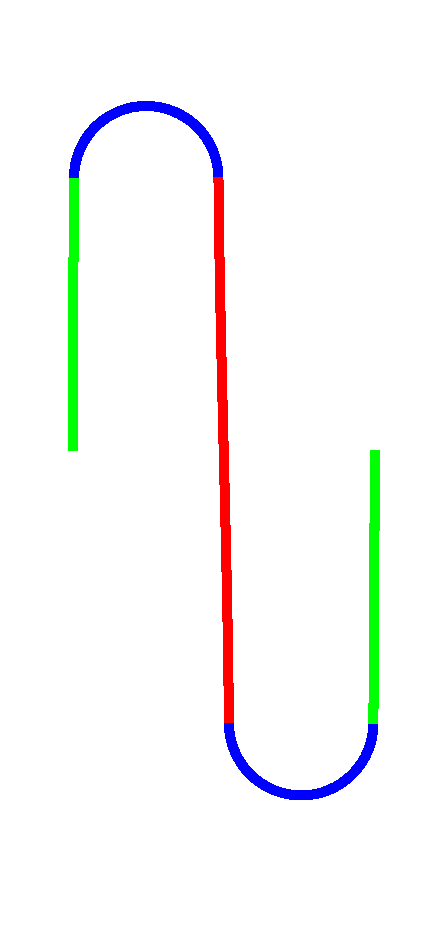
\includegraphics[width=0.25\linewidth]{OPT1.eps}
	\caption{单单元蛇形结构,相同颜色的条带优化过程中保持厚度相同}
	\label{fig:OPT1}
\end{figure}
、
\begin{table}
	\centering
	\caption{优化后的蛇形条带($n_c=1$)的厚度}
	\begin{tabular}{ll}
		\toprule
		临界交换高度及交换载荷          & 优化后宽厚比$w/t$   \\
		\midrule
		$\alpha=3,\pi_{\mathrm{cr}}=0.03$   & $w/t_1=11.86,\quad  w/t_2=15.00$ \\
		$\alpha=3,\pi_{\mathrm{cr}}=0.04$   & $w/t_1=9.90,\quad~~ w/t_2=13.06$    \\
		$\alpha=2,\pi_{\mathrm{cr}}=0.03$   & $w/t_1=11.66,\quad w/t_2=11.75$    \\
%		$\alpha=2,\pi_{\mathrm{cr}}=0.04$   & $w/t_1=,\quad w/t_2=$  \\
		\bottomrule
	\end{tabular}
	\label{tab:three-line}
\end{table}
\subsection{双单元蛇形结构的屈曲模态调控}
对单元数$n_c=2$的蛇形结构屈曲后同时具有S模态和M模态,如图~\ref{fig:OPT_1}所示。不同于单单元蛇形结构,多单元蛇形结构在不同结构高度$\alpha$下,S模态对应的临界载荷总小于M模态出现所需的最小载荷。因此,双单元蛇形结构发生平面失稳后总表现为S模态。本小节的优化目标为:在保持结构对称性的前提下,通过优化不同直线型条带的高度,实现S模态与M模态的顺序交换,即M模态出现所需的最小位移载荷小于S模态。
\begin{figure}
	\centering
	\subcaptionbox{双单元蛇形结构的S模态的$x-y$平面投影图(上)与M模态投影图(下)\label{fig:OPT_1}}
	{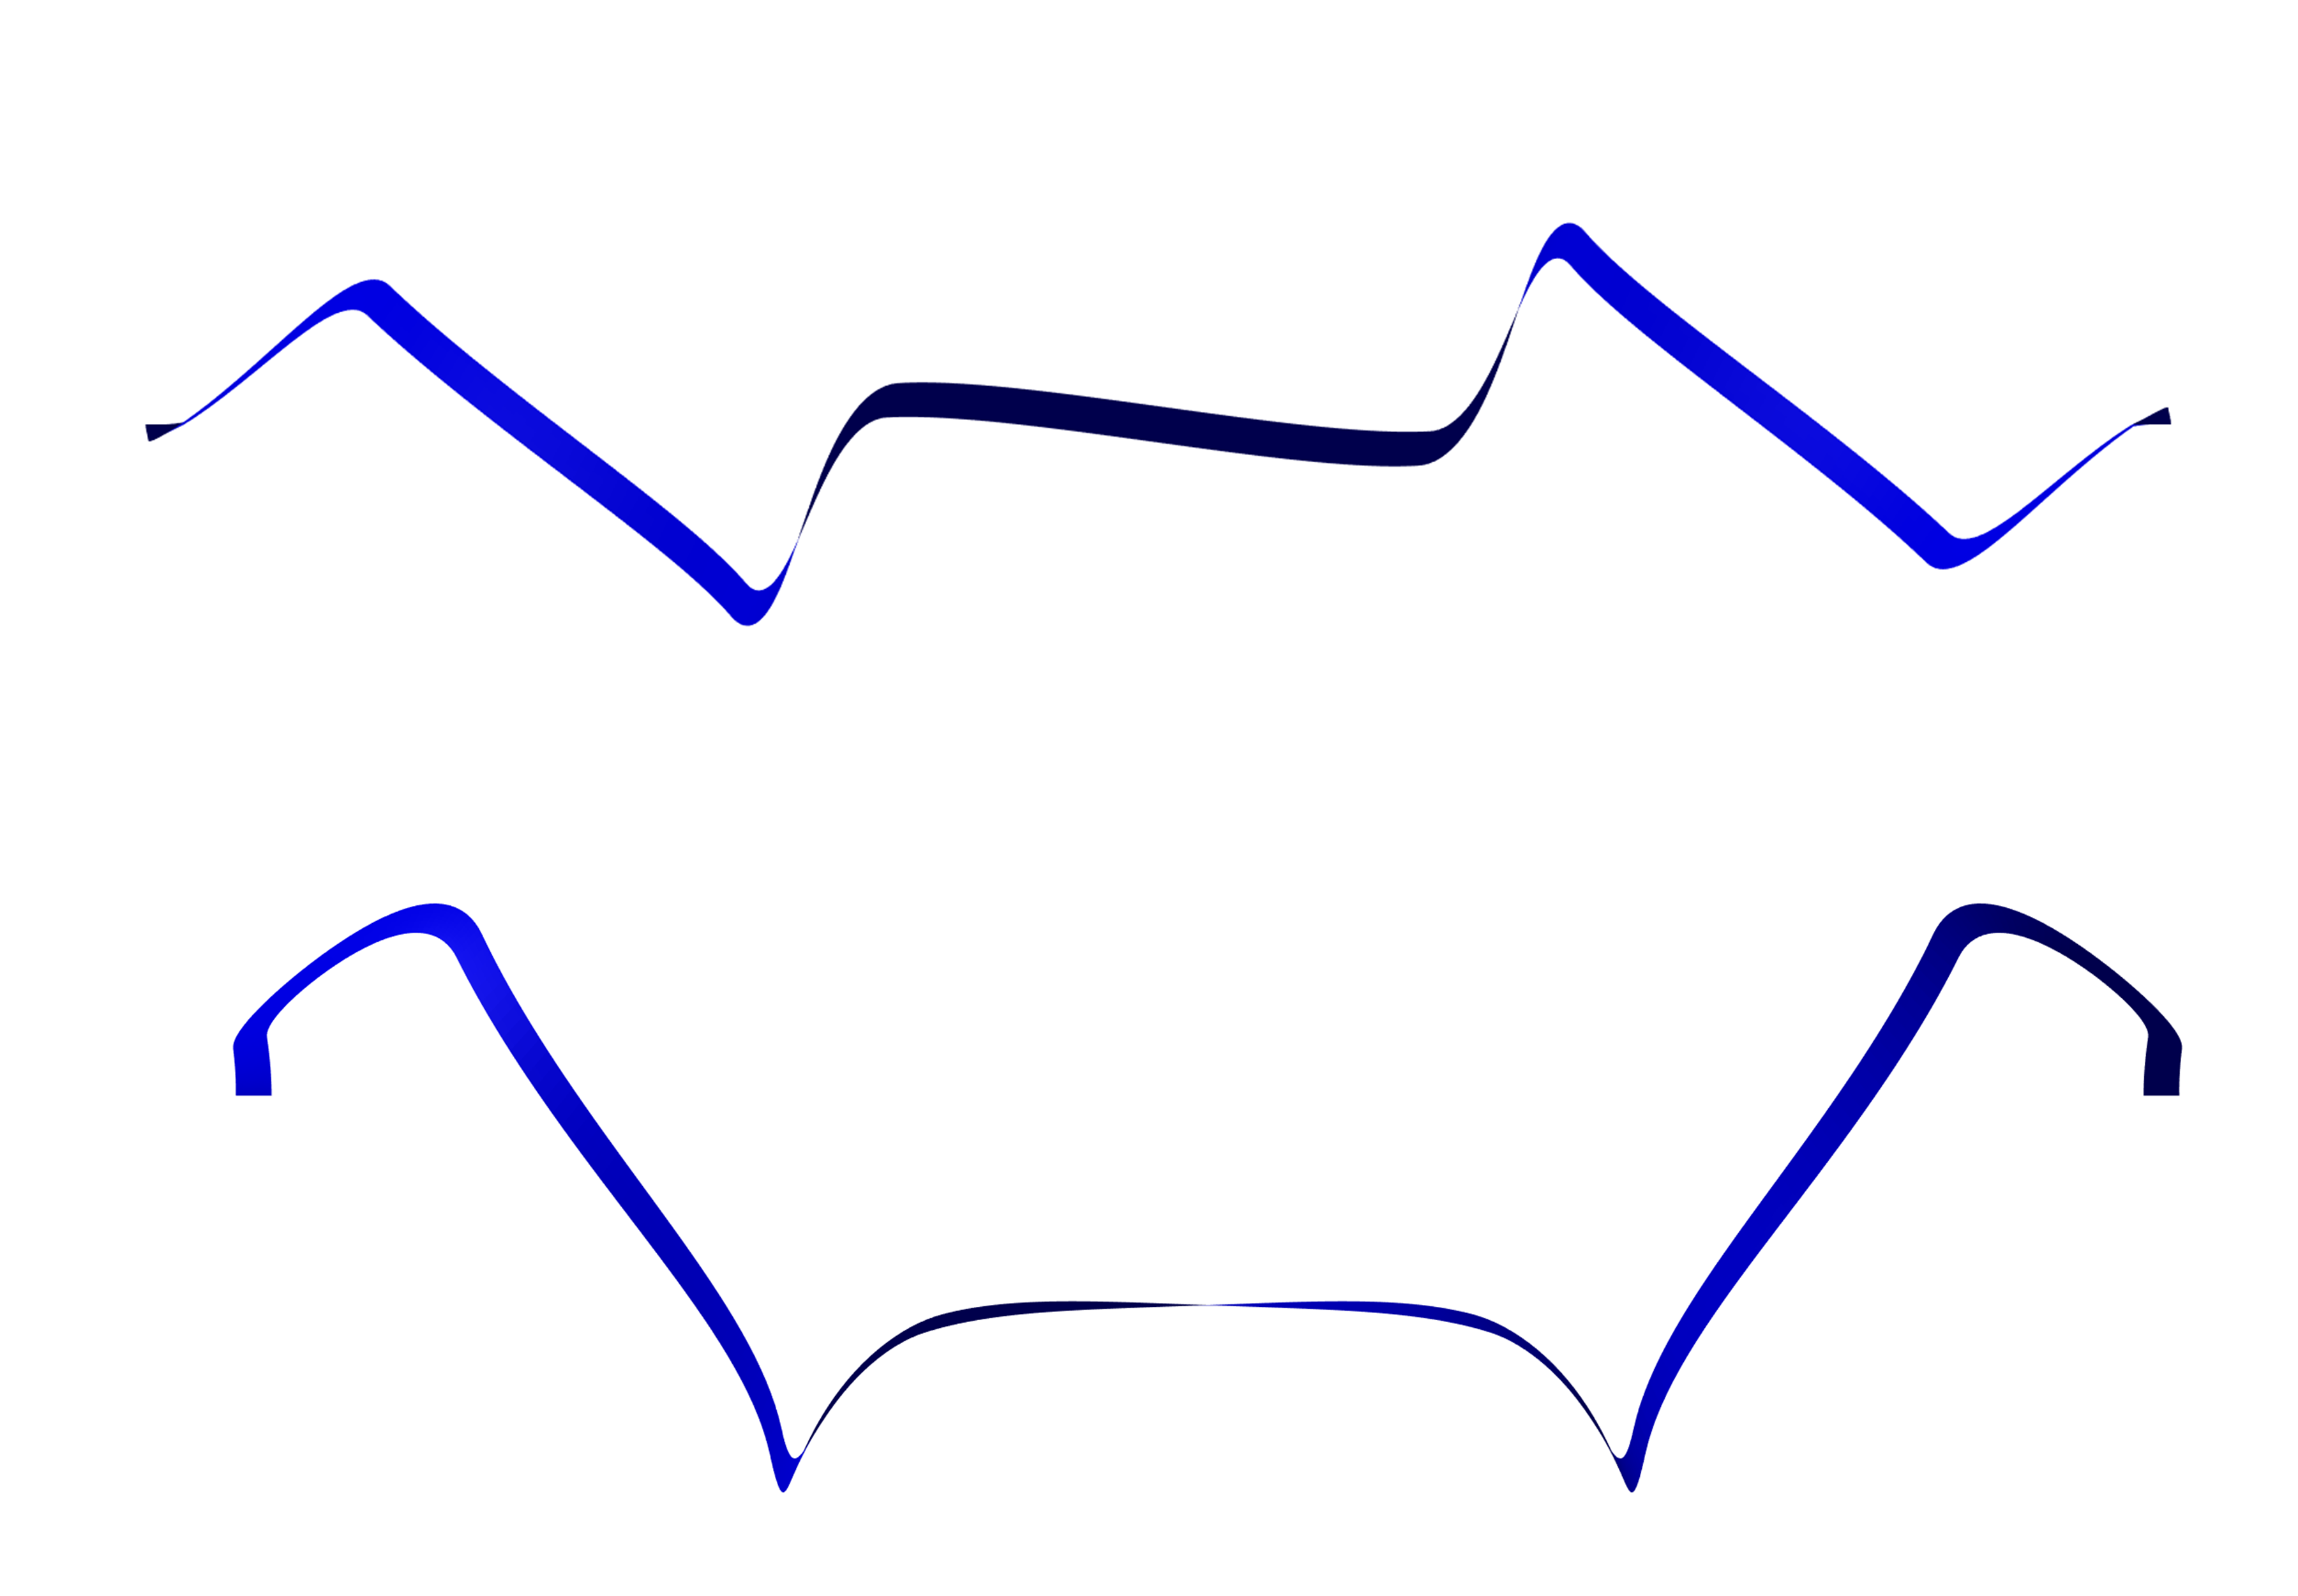
\includegraphics[width=0.45\linewidth]{OPT_1.png}}
	\subcaptionbox{优化后双单元蛇形结构构形\label{fig:OPT_Schematics}}
	{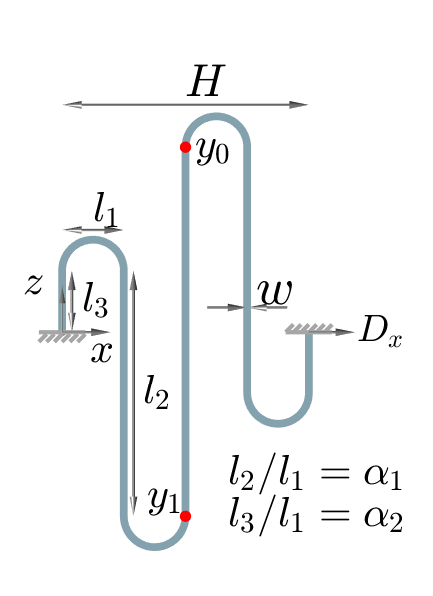
\includegraphics[width=0.3\linewidth]{OPT_Schematics.eps}}\\
	\caption{未优化前双单元蛇形结构的S模态和M模态以及优化后双单元蛇形结构}
	\label{fig:OPT_Intro}
\end{figure}

本处优化参数为直线型条带的无量纲高度,分别为图~\ref{fig:OPT_Schematics}中左起第一段直条带无量纲长度$l_3/l_1$和第二段直线条带无量纲长度$l_2/l_1$,为了保持结构的反对称性不变,最后一段直条带无量纲长度为$l_3/l_1$,倒数第二段直条带为$l_2/l_1$。最中间直条带的长度由其他直条带长度唯一确定,长度为$2\left(l_2-l_3\right)$。另外,为使优化求解器可以根据优化过程中出现的分岔点数量来自主决定下一优化步所需延拓区间的长度,这里将延拓区间的长度设优化参数,以保证在最终的优化结果中,延拓区间内只存在两个分岔点,对应S模态和M模态。综上所述,本优化问题的优化参数为三个,分别是第一段直条带长度$\alpha_2$和第二段直条带长度$\alpha_1$,以及延拓区间长度。

上一节指出在每一优化步中,参数延拓完成后需要判断所得分岔点对应的屈曲模态。为了区分分岔点对应的屈曲模态,分别向分岔支进行延拓任意固定步数(本文延拓$50$步),取出第$50$步计算得到的平衡解来给出图~\ref{fig:OPT_Schematics}中红色标注点$y$方向的位移,分别为$y_0$,$y_1$。该两点为蛇形结构上互为反对称的两点,从图~\ref{fig:OPT_1}中可以看出,对于S模态而言,结构上互为反对称的两点$y$方向位移大小相同,方向相反。而M模态上互为反对称的两点$y$方向位移,大小相同方向同向。因此可通过位移$y_1$,$y_2$之和来区分不同模态,若$y_1+y_2>0$,则所对应模态为M模态,若$y_1+y_2=0$,那么对应的模态为S模态。

为了实现双单元结构屈曲模态的交换,目标函数的误差度量项应为
\begin{equation}
	E=\pi_{1}-\pi_{2}+\mathrm{c}
	\label{eq:Error term2}
\end{equation}
式中$\pi_{1}$,$\pi_{2}$分别为M模态和S模态对应的分岔点位置。当两个分岔点位置相同时,即$\pi_{1}-\pi_{2}=0$,对应的优化参数为临界交换参数。通过设置一个很小的正数$\mathrm{c}$,用以确保当优化参数取得极小值零时,蛇形结构的一阶屈曲模态为M模态。

优化结果如图~\ref{fig:Phase_RB}所示,该图给出了在不同无量纲高度$\alpha_1$,$\alpha_2$组合下,双单元蛇形结构的一阶屈曲模态,若优化参数$\alpha_1$,$\alpha_2$落入红色区域,那么优化后蛇形结构的一阶屈曲模态为M模态,即相比于优化前,屈曲模态发生了交换;若优化参数$\alpha_1$,$\alpha_2$落入蓝色区域,那么其一阶屈曲模态仍为S模态。图~\ref{fig:Phase_RB}中红蓝区域的交界为临界参数,该交界上两分岔点重合。
\begin{figure}
	\centering
	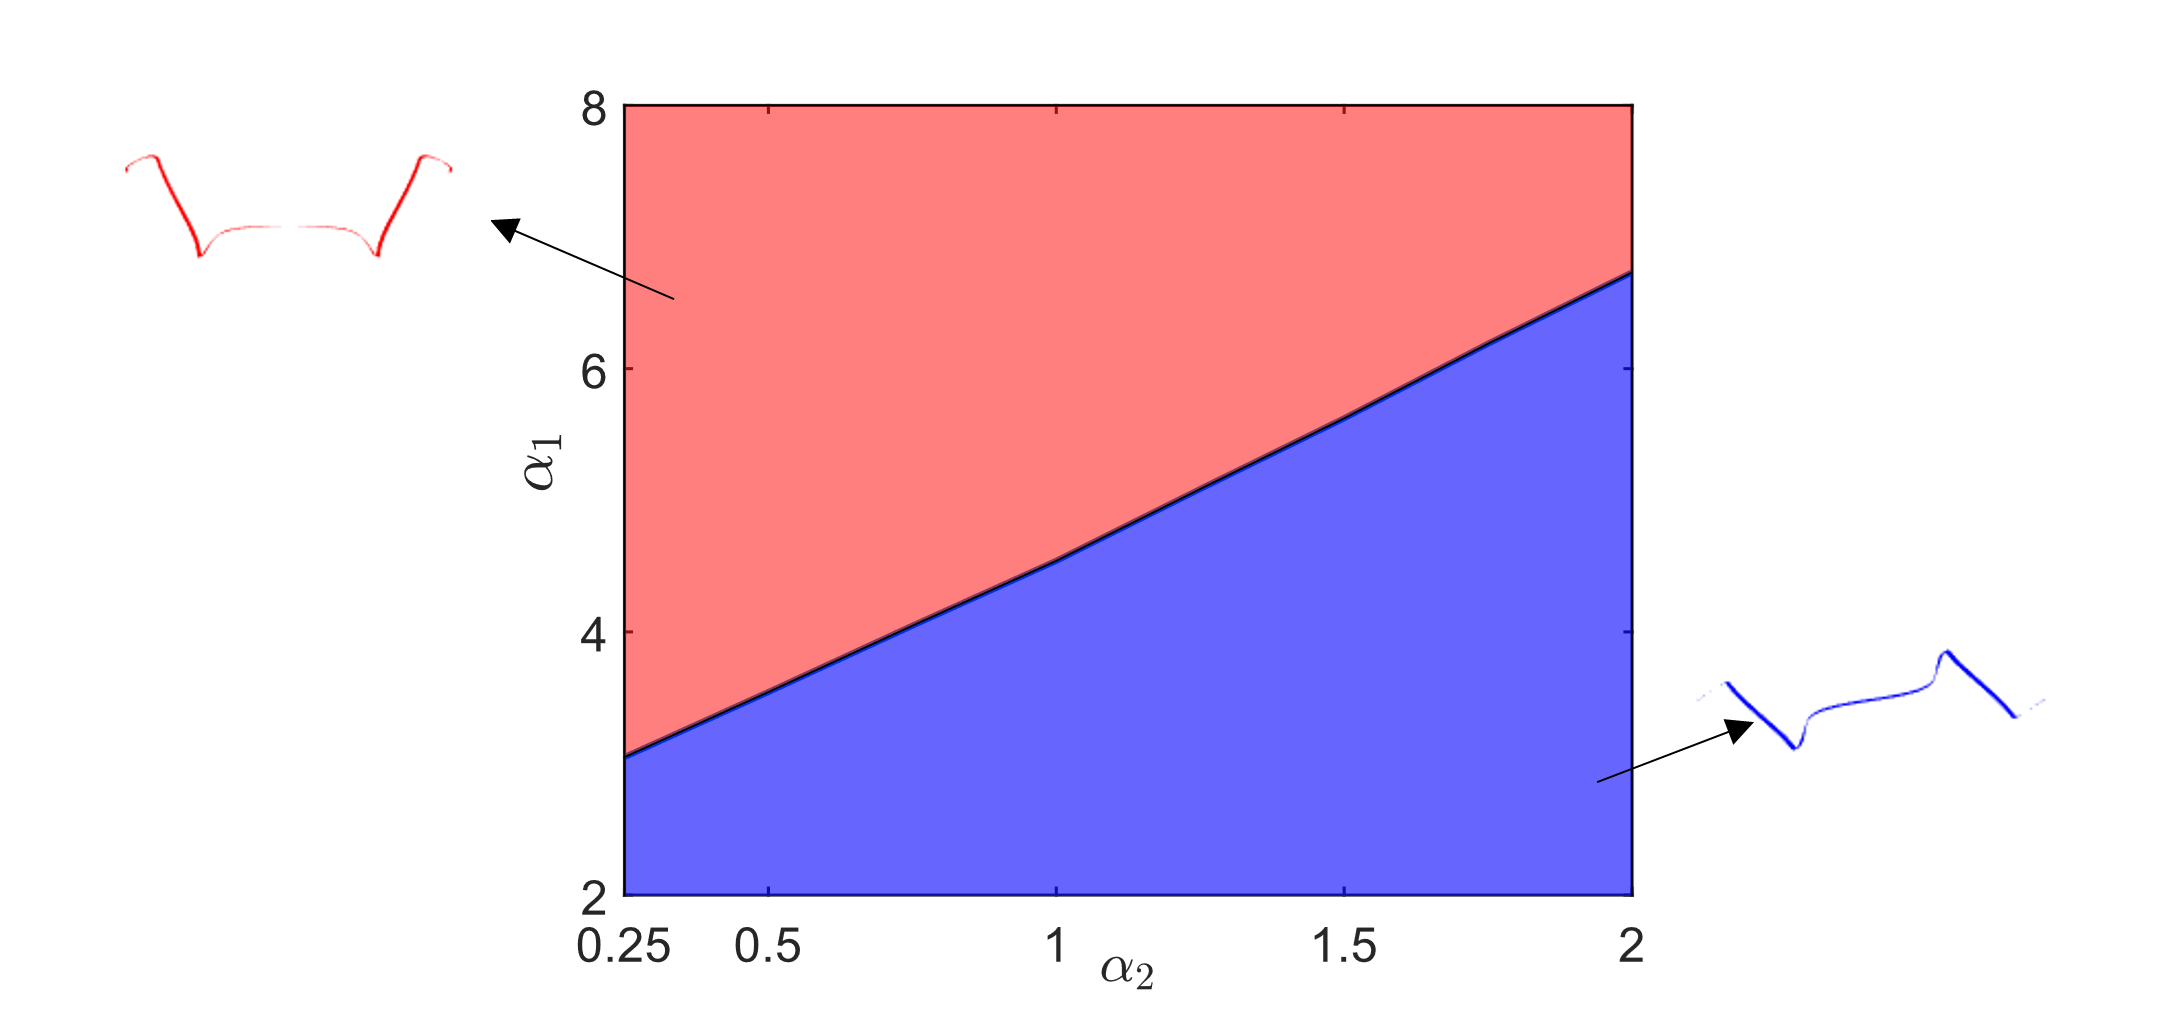
\includegraphics[width=1\linewidth]{Phase_RB.png}
	\caption{优化后蛇形结构的参数$\alpha_1,\alpha_2$落入蓝色区域,其一阶屈曲模态为S模态;红色区域为M模态}
	\label{fig:Phase_RB}
\end{figure}

为了研究优化后蛇形结构的模态交换过程,本文以固定$\alpha_2=1$为例,研究蛇形结构屈曲模态随$\alpha_1$变化的交换过程。根据优化结果可知,$\alpha_1=4.54$为临界交换点,若$\alpha_1>4.54$,那么优化后结构的一阶屈曲模态为M模态,若$\alpha_1<4.54$,那么优化后结构的一阶屈曲模态为S模态。为了得到结构在该参数下详细的模态交换过程,这里在临界交换点附近分别取$\alpha_1=4,4.75,5$三个参数,来绘制相应的分岔曲线,如图~\ref{fig:OPT2_Bifurcation}(a-c)所示,分别代表屈曲模态交换前,分岔点位置发生交换而稳定性未完全交换,屈曲模态完全交换后的分岔曲线。
\begin{figure}
	\centering
	\subcaptionbox{$\alpha_1=4$下的分岔图\label{fig:OPT2_1}}
	{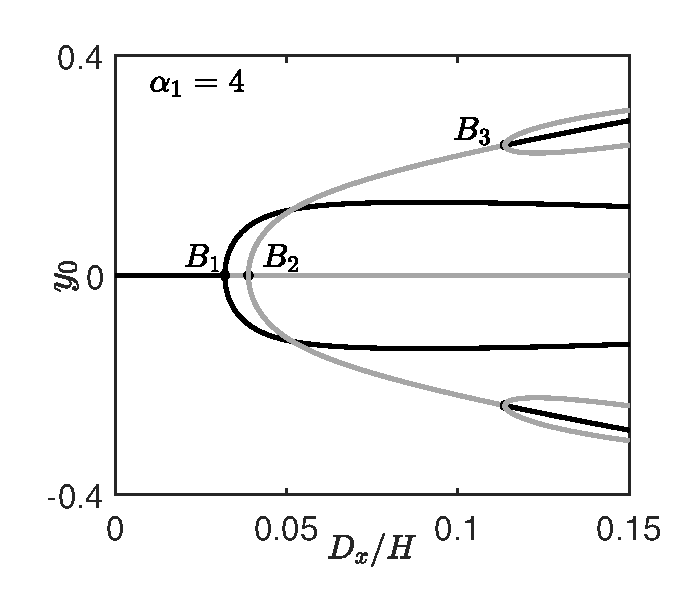
\includegraphics[width=0.495\linewidth]{OPT2_1.eps}}
	\subcaptionbox{$\alpha_1=4.75$下的分岔图\label{fig:OPT2_2}}
	{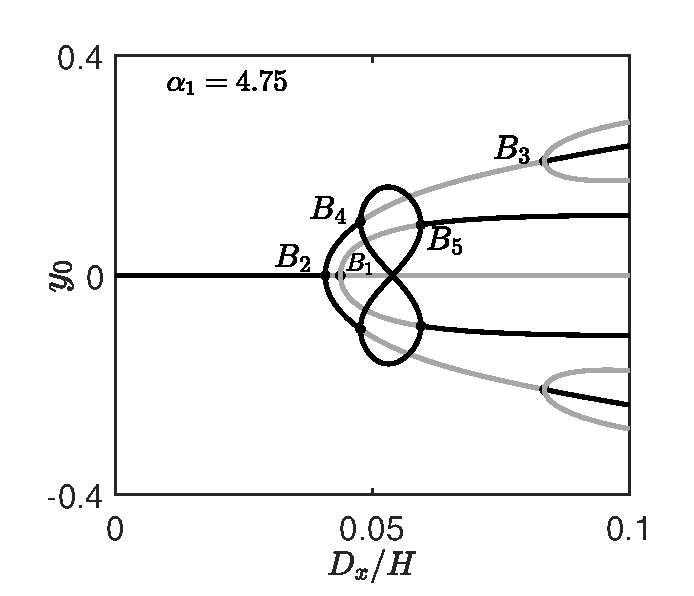
\includegraphics[width=0.495\linewidth]{OPT2_2.eps}}\\
	\subcaptionbox{$\alpha_1=5.75$下的分岔图\label{fig:OPT2_3}}
    {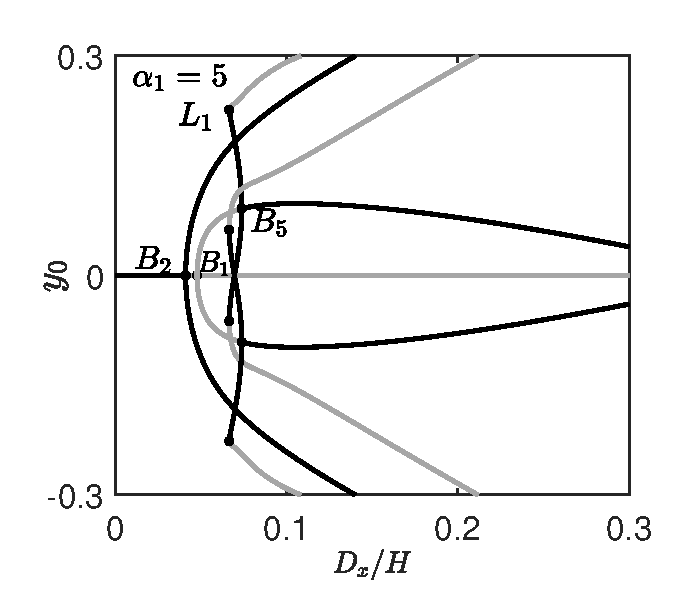
\includegraphics[width=0.495\linewidth]{OPT2_3.eps}}
    \subcaptionbox{分岔图(a-c)中分岔点随$\alpha_1$的轨迹\label{fig:OPT2_4}}
    {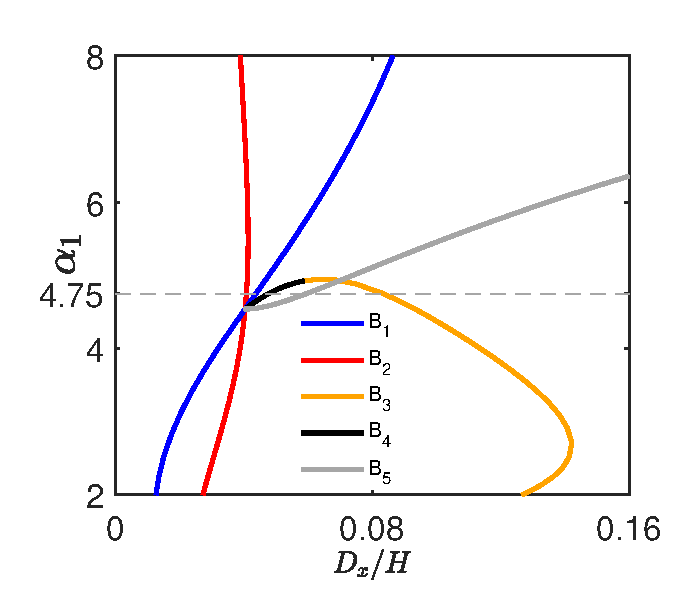
\includegraphics[width=0.495\linewidth]{OPT2_4.eps}}\\
    \subcaptionbox{不同$\alpha_1$下一阶屈曲模态(左)及二阶屈曲模态(右)\label{fig:OPT2_R}}
    {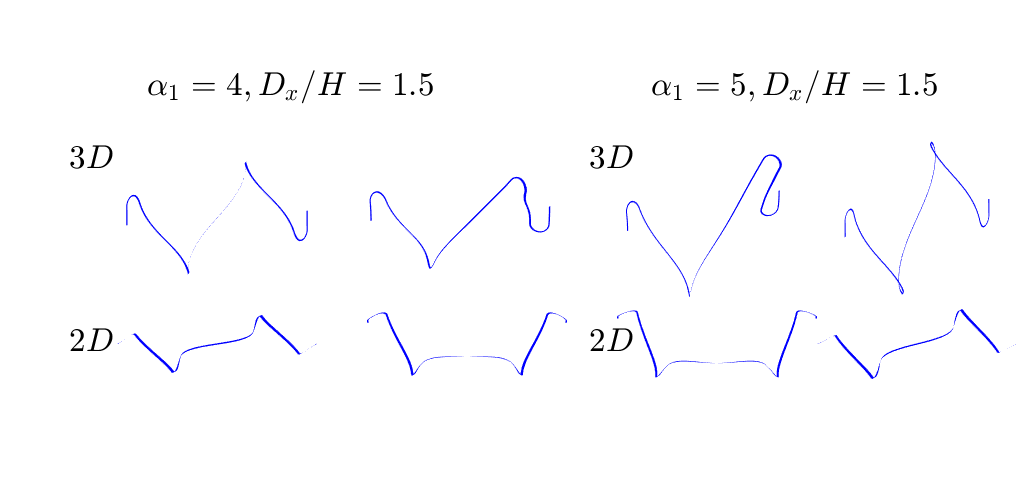
\includegraphics[width=1\linewidth]{OPT2_R.eps}}    
    \caption{$\alpha_2=1$,不同$\alpha_1$	​
    	取值下双单元蛇形结构的分岔图,包括分岔点的轨迹以及不同参数下的一阶屈曲模态和二阶屈曲模态}	
	\label{fig:OPT2_Bifurcation}
\end{figure}

图~\ref{fig:OPT2_Bifurcation}的分岔图中,分岔点$B_1$,$B_2$分别对应S模态和M模态的分岔点,图~\ref{fig:OPT2_1}中,分岔点$B_1$在分岔点$B_2$之前,因此结构失稳后首先出现S模态。而分岔点$B_2$的分岔支(对应M模态)在分岔点$B_3$之前为不稳定解,在分岔点$B_3$之后,M模态和S模态同时存在。图 ~\ref{fig:OPT2_2}为$\alpha_1=4.75$的分岔图,该分岔图中分岔点$B_2$先于分岔点$B_1$,当达到失稳临界载荷时,结构会屈曲为M模态。M模态对应的平衡解在经过超临界分岔点$B_4$变为非稳定解,但随后经过亚临界分岔点$B_3$后重新恢复为稳定平衡解。在平面解分支($y_0=0$)上分岔点$B_2$之后存在分岔点$B_1$,从该分岔点分岔出一对不稳定的平衡分支,该分岔支在经过超临界分岔点$B_5$之后变为稳定分支,对应稳定的S模态。类似图~\ref{fig:SerpentineNc1Aniso10Phase}中$\alpha=2.346$,$n_c=1$的蛇形结构的分岔曲线,分岔点$B_4$和$B_5$共同构成一个闭合的环。如图~\ref{fig:OPT2_3}所示,随着$\alpha_1$的进一步增大,分岔点$B_4$和$B_5$相互融合,使得M模态对应的整个分岔支变为稳定分支。

图~\ref{fig:OPT2_4}为分岔图中各分岔点随$\alpha_1$的轨迹图,通过轨迹图可以确定模态交换的临界$\alpha_1=4.541$,同时可以看出二次分岔点$B_4$的在临界$\alpha_1$时出现,使得两个屈曲模态的平衡分支的稳定性发生了交换。从以上分岔分析可知,优化后蛇形结构的模态交换同样伴随着多重特征值分岔的出现,多重特征值分岔引发二次分岔点$B_4$,$B_5$的出现,使得S模态与M模态的平衡分支发生了稳定性交换。图~\ref{fig:OPT2_R}展示了$\alpha_1=4,D_x/H=1.5$以及$\alpha_1=5,D_x/H=1.5$对应的一阶屈曲模态(左起第一第三构形为一阶屈曲模态)和二阶屈曲模态(左起第二第四构形为二阶屈曲模态),进一步说明了大于临界$\alpha_1$的蛇形结构其一阶屈曲模态为M模态,小于临界$\alpha_1$的蛇形结构其一阶屈曲模态为S模态。
\subsection{三单元蛇形结构的屈曲模态调控}
本小节以三单元蛇形结构为例,来说明通过改变蛇形结构不同单元的厚度,可以有效调控其屈曲构形。具体而言,在后屈曲阶段,通过调控单元厚度可以抑制某些单元的形变,也可以鼓励某一单元发生更大的形变,这为蛇形结构在实际应用中的设计提供了重要的思路。

图~\ref{fig:OPT3}为单元厚度调节后的蛇形条带($n_c=3$)的屈曲构形及分岔图。在调节厚度的过程中,保持条带的宽度不变,通过改变条带厚度来改变条带截面的宽厚比。图~\ref{fig:OPT_NC3_1}中第$\rom{1}$行展示了蛇形单元在五种情况下的厚度分布。在第一种情况下,整个条带的厚度均匀分布,宽厚比$w/t$为$10$。在后面的几种蛇形条带中,总有一个单元宽厚比不为$10$,具体而言,用蓝色表示的单元宽厚比默认为$10$,而红色表示的单元宽厚比$w/t$等于$8$或者$12.5$。图~\ref{fig:OPT3_1}和图~\ref{fig:OPT3_2}分别为第一个单元宽厚比$w/t=12.5,8$的蛇形结构的分岔图。分岔图中平衡分岔支上标记点处的屈曲构形的二维投影如图~\ref{fig:OPT_NC3_1}中第(b-c)列所示。以图~\ref{fig:OPT_NC3_1}中第(a)列的原构形为基准,第一个单元厚度增大后,如图~\ref{fig:OPT_NC3_1}中第(c)列所示,该单元屈曲后的面外形变被抑制;在减薄第一个单元厚度的情况下,如图~\ref{fig:OPT_NC3_1}中第(b)列所示,该单元的面外变形被放大。分岔图~\ref{fig:OPT3_1}和图~\ref{fig:OPT3_2}表明,当载荷超过临界值$B_1$时,结构屈曲为S模态(~\blacksquare~/~\blackdiamond~),而M模态(~\bltriangle~/~\Rtriangle~)对应的平衡分支不与平面解相连,该分支在拐点$L_1$之后变为稳定解。对蛇形结构($n_c=3$)的第一个单元厚度调控后,整个结构失去了反对称性,即破坏了可逆对称性,关系式\eqref{eq:R1R2}失效。
\begin{figure}
	\centering
	\subcaptionbox{第一个蛇形单元$w/t=12.5$下的分岔图\label{fig:OPT3_1}}
	{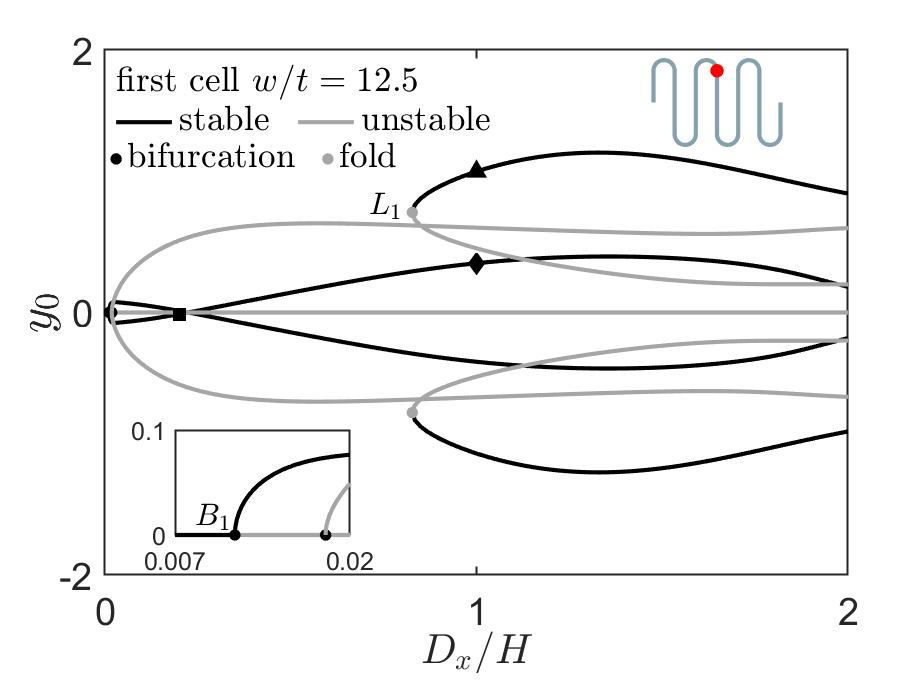
\includegraphics[width=0.495\linewidth]{OPT3_1.eps}}
	\subcaptionbox{第一个蛇形单元$w/t=8$下的分岔图\label{fig:OPT3_2}}
	{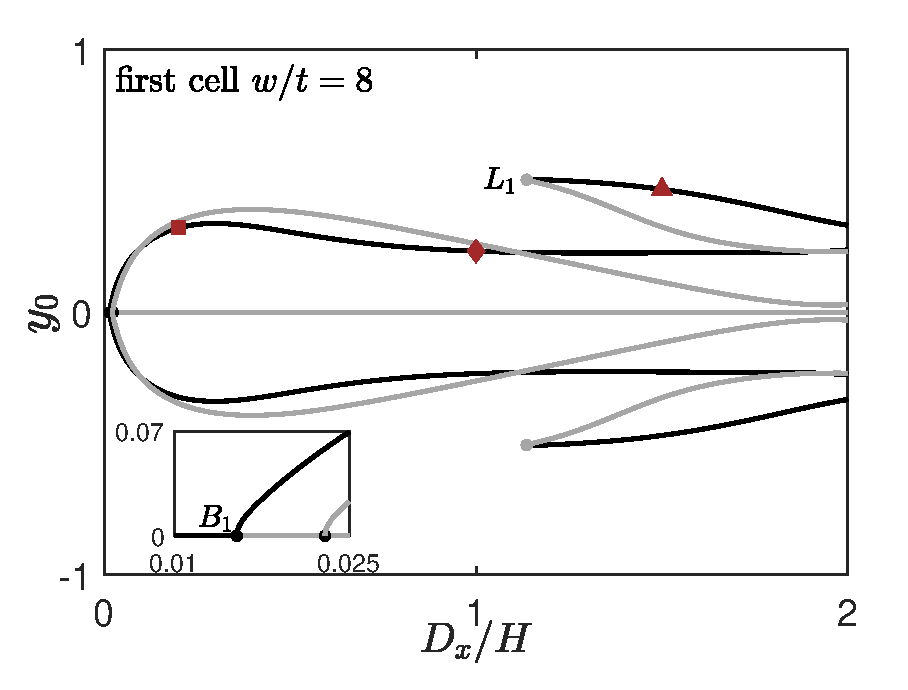
\includegraphics[width=0.495\linewidth]{OPT3_2.eps}}\\
	\subcaptionbox{第二个蛇形单元$w/t=12.5$\label{fig:OPT3_3}}
	{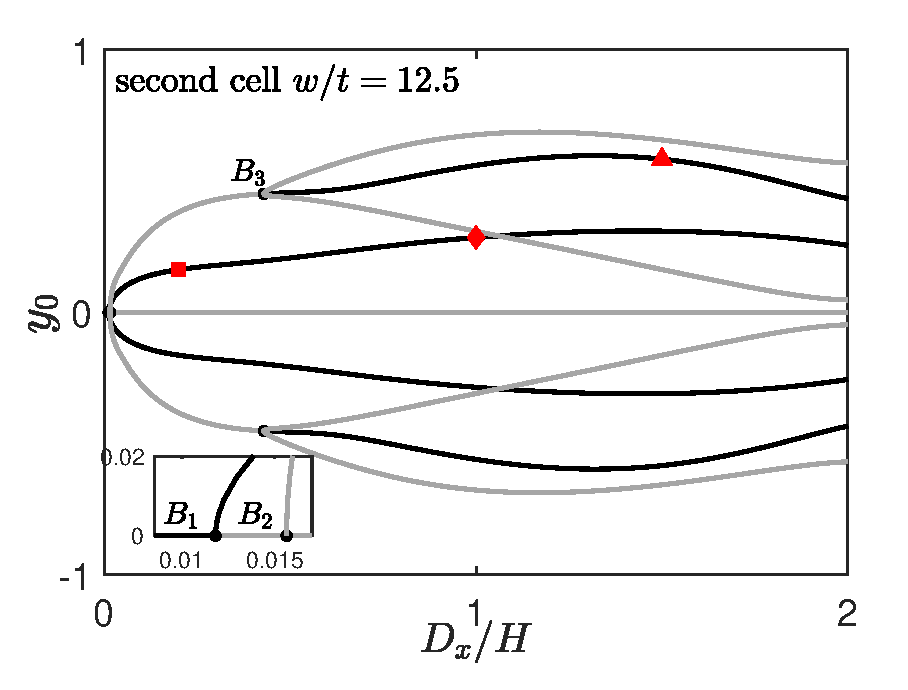
\includegraphics[width=0.495\linewidth]{OPT3_3.eps}}
	\subcaptionbox{第二个蛇形单元$w/t=8$时的分岔图\label{fig:OPT3_4}}
	{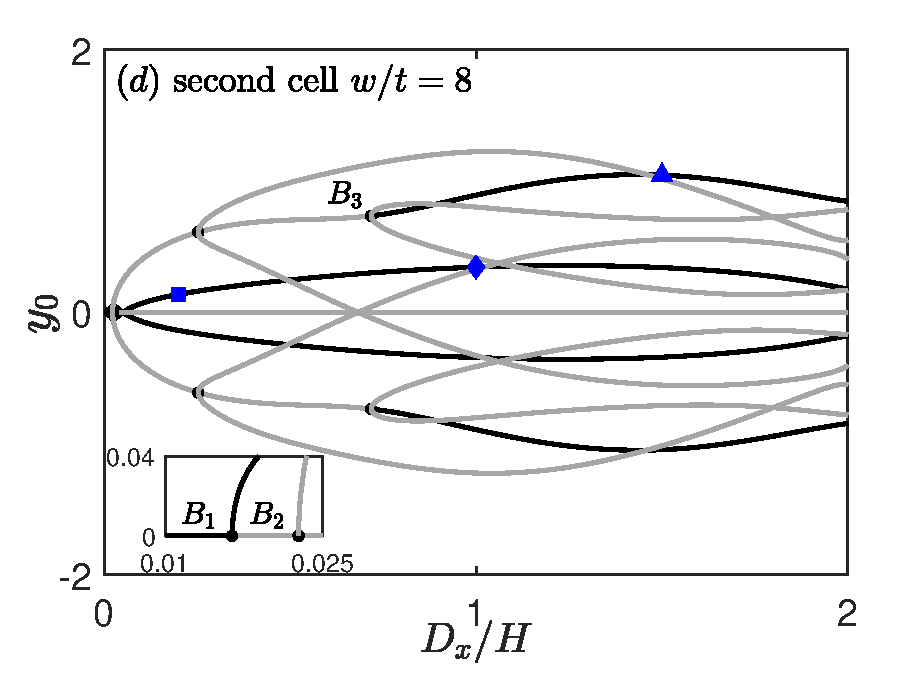
\includegraphics[width=0.495\linewidth]{OPT3_4.eps}}\\
	\subcaptionbox{厚度优化后的结构屈曲构形。红色表示的单元为厚度经过调节后的单元\label{fig:OPT_NC3_1}}
	{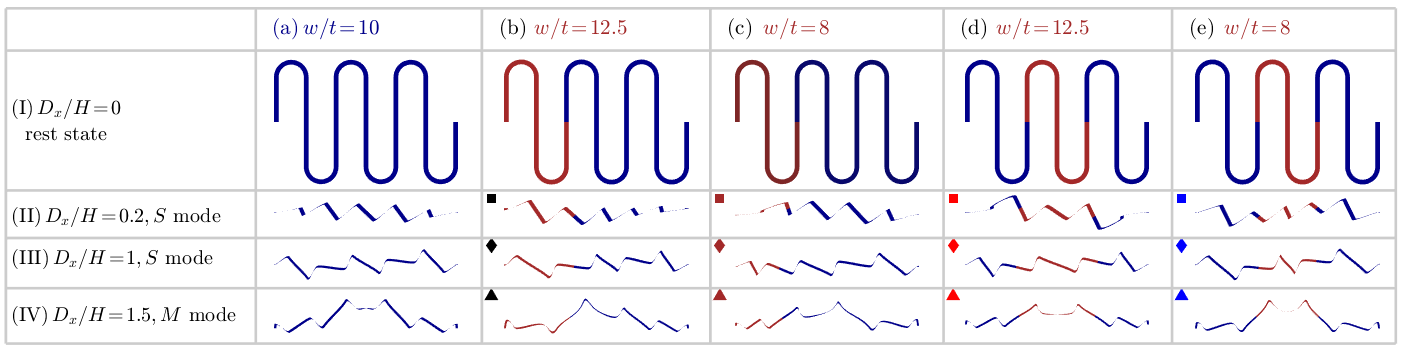
\includegraphics[width=1\linewidth]{OPT_NC3_1.png}}
	\caption{厚度优化后$n_c=3$的蛇形结构的屈曲构形及分岔图}	
	\label{fig:OPT3}
\end{figure}

图~\ref{fig:OPT3_3}和图~\ref{fig:OPT3_4}为调控中间单元厚度后的蛇形结构($n_c=3$)的分岔图,调控后第二个单元的宽厚比$w/t$分别为$12.5$和$8$。这种情形下,调控后的蛇形结构仍然保持反对称性,因此可逆对称性的关系式\eqref{eq:R1R2}仍然满足,平衡构形仍成对(自可逆对)或成组(平衡构形组)存在。在分岔点$B_1$后,调控后的蛇形结构发生面外屈曲,屈曲模态为S模态,平面平衡分支上第二个分岔点$B_2$分岔出一对不稳定的平衡分支,当该分岔支穿过$B_3$时,变为稳定解,对应M模态。从图~\ref{fig:OPT_NC3_1}中第(d-e)列可以看出增大厚度会抑制屈曲形变,减小厚度会放大屈曲形变。


